\chapter{緒論}
\renewcommand{\baselinestretch}{10.0} %設定行距
\pagenumbering{arabic} %設定頁號阿拉伯數字
\setcounter{page}{1}  %設定頁數
\fontsize{14pt}{2.5pt}\sectionef
\section{研究動機與背景}
材料分析軟體的應用在機械領域愈來越廣泛,能夠將繪製零件進行分析,但卻鮮少人知道材料分析是怎麼進行的,背後所引用的代碼、原理的東西。本專題研究方向將由四足機器人(圖.\ref{fig.冰球機})作為設計主題,提供所需參數,將有限元素分析(圖.\ref{fig.模擬冰球機})的公式套入並計算,對建模進行力學分析,透過本專題了解分析軟體求解的過程(圖.\ref{fig.pong_gym})。\\

\begin{figure}[hbt!]
\begin{center}
\includegraphics[angle=90,width=10cm]{冰球機}
\caption{\Large 實體的冰球機}\label{fig.冰球機}
\end{center}
\end{figure}
\begin{figure}[hbt!]
\begin{center}
\includegraphics[angle=90,width=10cm]{origin}
\caption{\Large 虛擬環境簡化後的冰球機}\label{fig.模擬冰球機}
\end{center}
\end{figure}
\begin{figure}[hbt!]
\begin{center}
\includegraphics[height=8cm]{pong_gym}
\caption{\Large Gym的Pong game}\label{fig.pong_gym}
\end{center}
\end{figure}


\section{研究目的}
本研究分三大部分,第一運用OpenAI Gym裡內建編譯的ATARI 2600遊戲Pong-v0,來作為訓練環境,加上強化學習的理論,測試不同演算法參數以訓練出最佳化的對打系統,第二將整個簡化後冰球機導入CoppilaSim模擬環境並嘗試進行虛擬訓練,成為優化的對打機電系統。第三則是嘗試透過架設伺服器與虛擬環境結合。\\
 
透過簡化實體冰球機並導入虛擬環境,進行虛擬訓練,使用Gym的Pong當作對應的2D虛擬訓練環境,測試算法和訓練效果,篩選適合的算法與參數。\\

建置CoppilaSim模擬環境,嘗試將2D訓練概念套用到3D環境進行測試,加入電腦視覺與RemoteAPI,電腦視覺抓取球與擊錘的位置,透過RemoteAPI進行遠端控制,在3D環境測試算法可確保後續套用到實體機器上的可行性。\\
 
 再透過架設伺服器與虛擬環境結合:讓虛擬環境的影像透過網伺服器串流影像供使用者遠端進行操控虛擬環境的擊錘進行打球,或是提供多人進行觀看對打影像。
\begin{figure}[hbt!]
\begin{center}
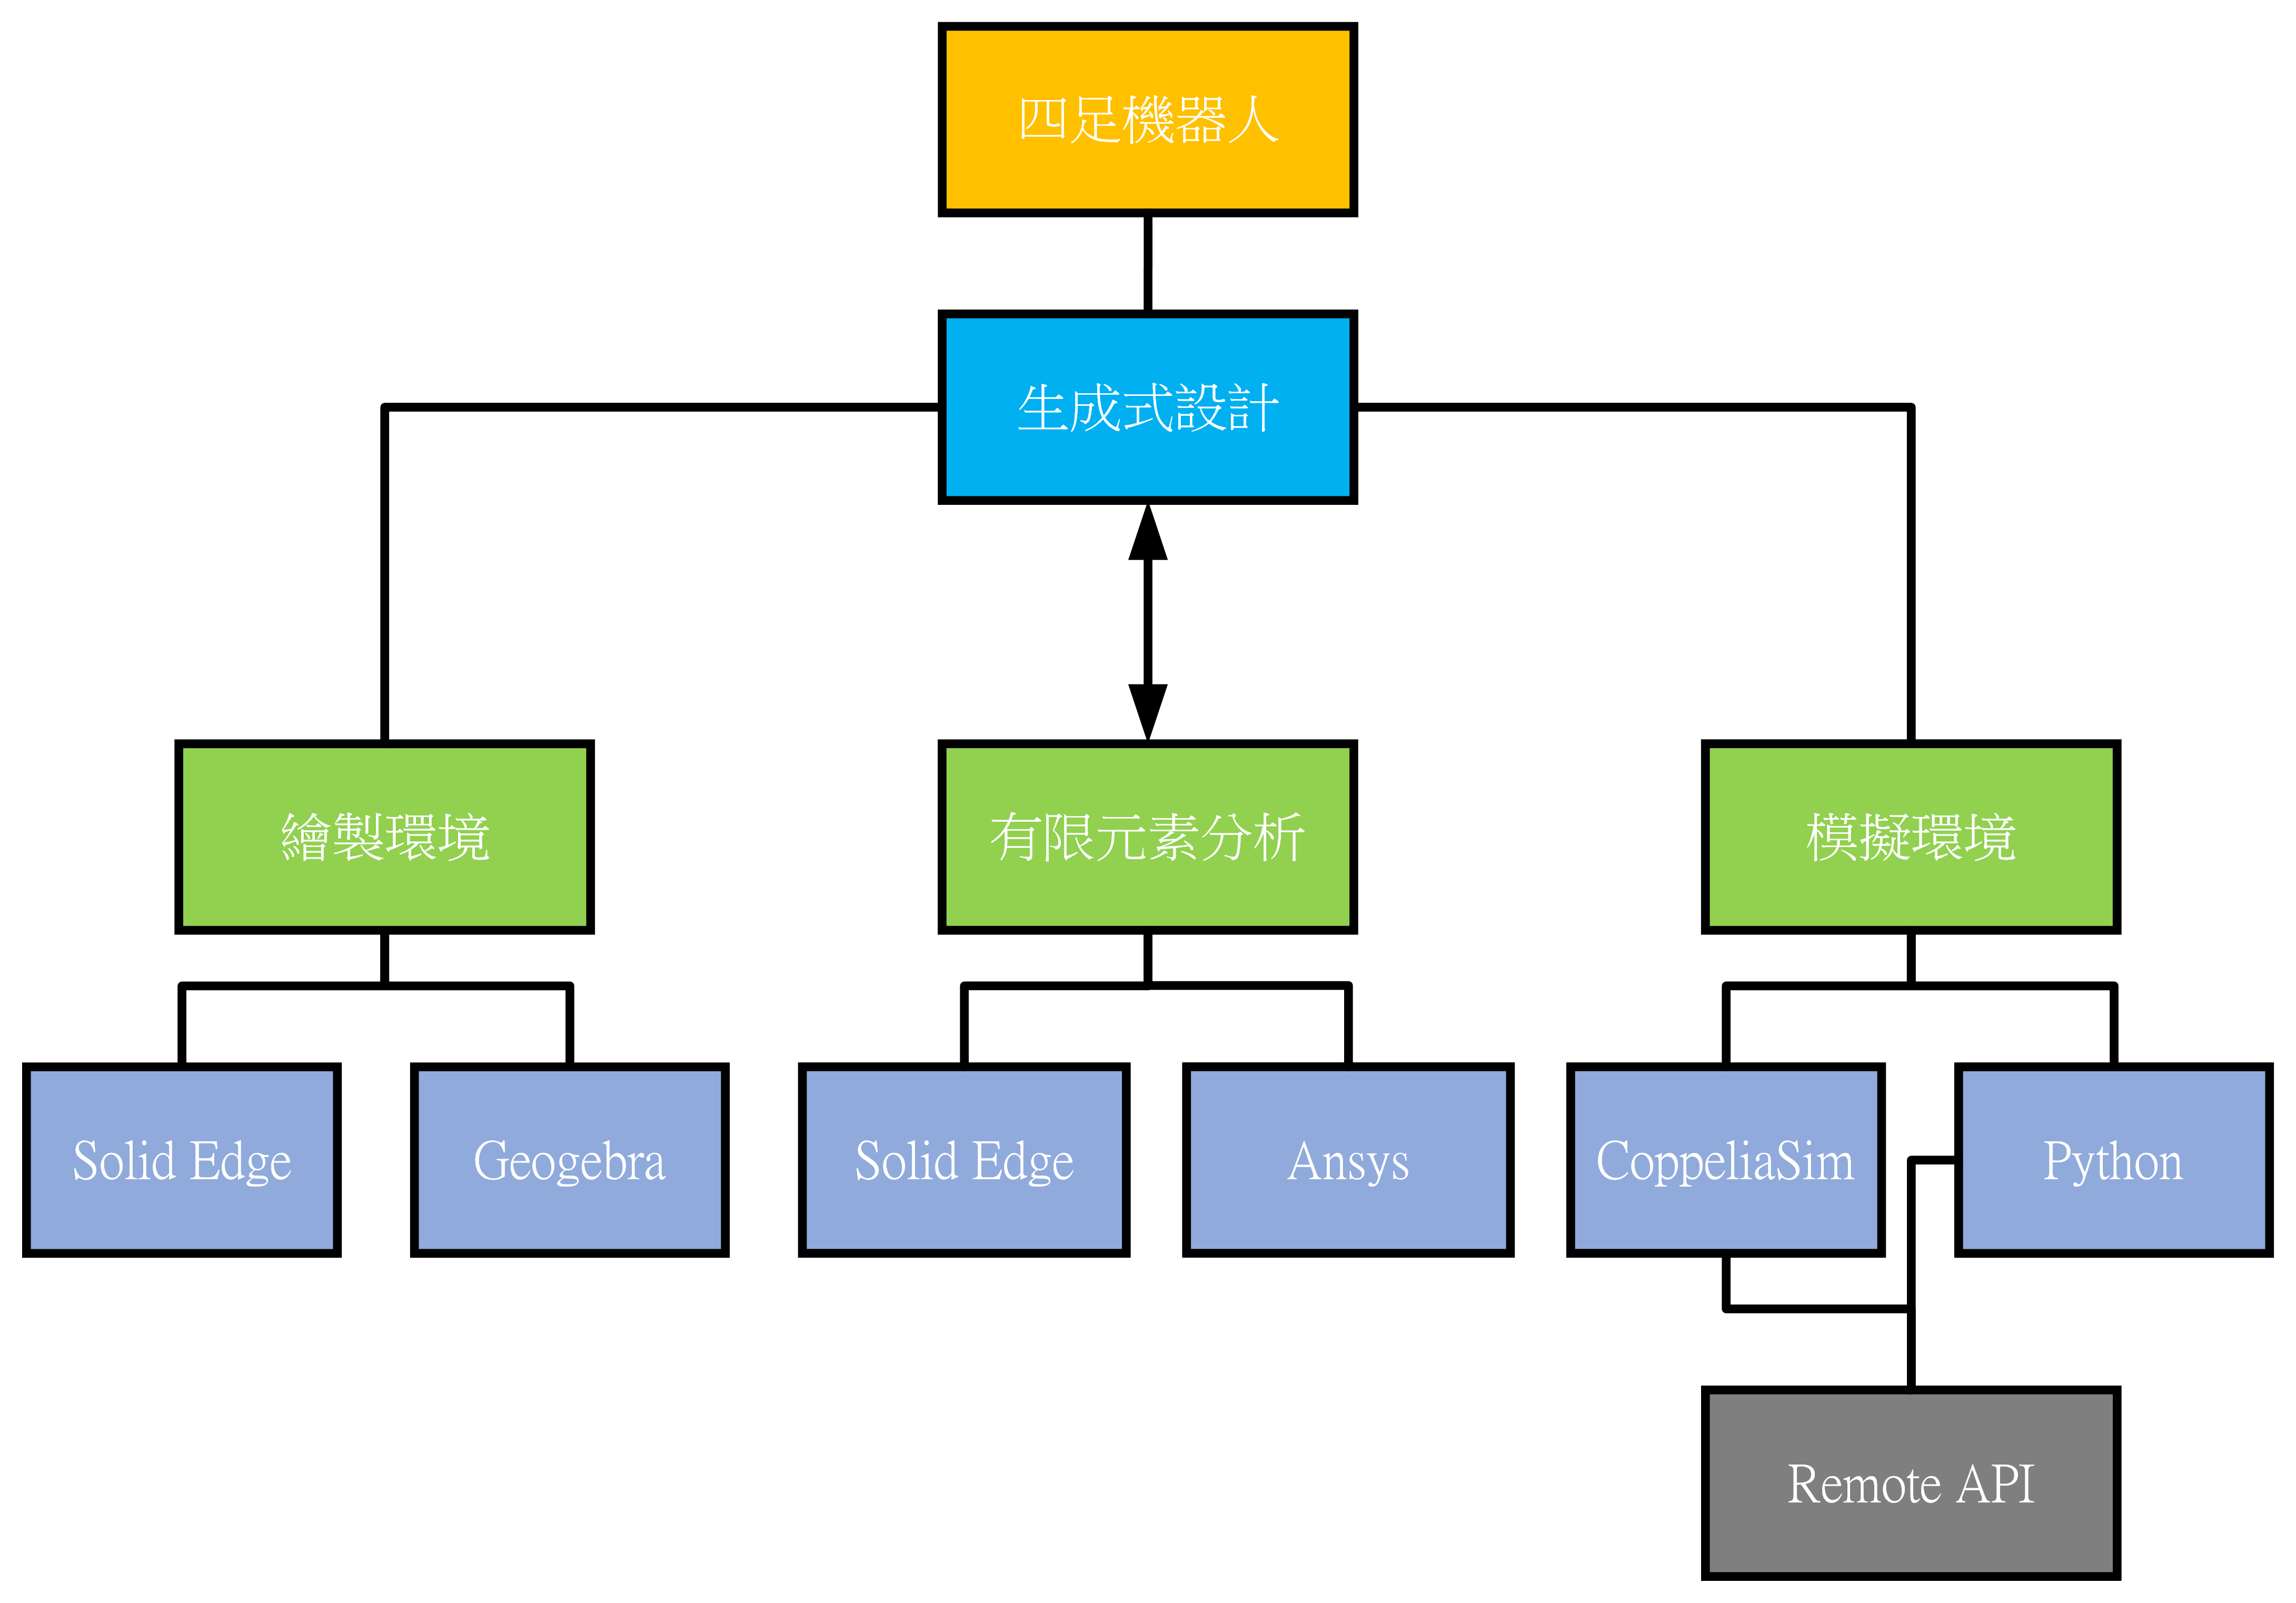
\includegraphics[width=15cm]{研究架構}
\caption{\Large 研究架構 }
\label{研究架構 }
\end{center}
\end{figure}
\section{研究方法}
此專題希望能利用現有完成的機械學習的算法,能發展成虛擬訓練,再將訓練完的機器學習應用到虛擬環境或是實體機電系統,並透過伺服器將影像串流提供玩家網頁介面進行遠端操控,同時提供多人觀看及時的比賽影像,將整個冰球機的控制和使用者間有更完善串聯,機電系統的部分達到最優化控制和虛實整合的應用。
\section{未來展望}
 Pong game 的遊戲規則簡單,透過擊錘將球打入對方球門即得一分,只要其中一方得21分就結束該局。擊錘只能沿單方向來回移動來進行防守和進攻。\\
遊戲規則如下:
\begin{enumerate}
\item 球打入敵方即得一分。
\item 擊錘只單一方向移動。
\item 最快贏得21分者獲勝,並結束該局遊戲。
\end{enumerate}

\renewcommand{\baselinestretch}{0.5} %設定行距
